%!TEX root = main.tex

\chapter{Background}
\label{background}


%!TEX root = main.tex

% NOTES:
%   * There is a shift to accelerator design
%   * CPUs are inefficient
%   * Fixed accelerators are hard to program
%   * Alternative is FPGA/CGRA
%   * There are challenges with programming FPGA/CGRA
%   * HLS is one solution
%

\section{Why application specific accelerators?}
\label{background:accel}


Recent trends in technology scaling, the availability of large amounts of data, and novel algorithmic breakthroughs have spurred accelerator architecture research.
In a general-purpose microprocessor, the overhead of instruction processing is much higher than the actual operations performed by each instruction.
This overhead includes the necessary steps to fetch and decode the instructions, provide required operands for the instructions, and perform the necessary bookkeeping to ensure correctness when multiple instructions are executing in the microprocessor.
Conversely, application specific hardware are faster and lower in power consumption than general-purpose processors because they eliminate most of the overhead of a general purpose processor~\cite{chung_micro_2010, hameed_asplos_2010_understanding}.
Although fixed-function accelerators are more energy efficient than software running a general-purpose processor, they are not a suitable solution for applications that change frequently.
As an alternative to fixed-function accelerators, reconfigurable architectures like field-programmable gate arrays (FPGAs) and coarse-grain reconfigurable architectures (CGRAs) have received renewed interest from academic researchers and industry practitioners alike, primarily due to their potential performance and energy efficiency benefits over conventional CPUs.
For instance, FPGAs are now being used to accelerate web search in datacenters at Microsoft and Baidu~\cite{catapult, baidu}, Amazon now offers FPGA instances as part of AWS~\cite{awsf1}, and Intel has announced products like in-package Xeon-FPGA systems~\cite{harp} and FPGA-accelerated storage systems~\cite{nand_flash}. Similarly, several recent research prototypes~\cite{dyser, triggered_instruction, scaledeep, scnn, plasticine, cgra_me} have explored various kinds of CGRAs at different granularity. Growing use of such reconfigurable architectures has made them more available to programmers now than ever before.
Although the flexibility of reconfigurable architectures enables changing the application by reconfiguring the accelerator, their programmability is still a major obstacle for their wide spread use.

\section{System-Design Challenges}


Reconfigurable devices, usually, accelerates part of the application which contains regular control flow and abundant data parallelism to achieve high performance and efficiency~\cite{spatial_computation, trips, govindaraju_hpca_2011}.
They can exploit: 1)multiple levels of nested parallelism, 2)data locality with custom data pipelines and 3)defining custom memory hierarchies.

Unfortunately, \textit{all the features that make reconfigurable architectures efficient also make them much more complex to program.}
For instance, in FPGAs, an accelerator design must account for the timing between pipelined signals and the physically limited compute and memory resources available on the target device.
It must also manage partitioning of data between local scratchpads and off-chip memory to achieve good data locality~\cite{gzip_2013_fpga}.

The combination of these complexities and market pressures, not the least
of which is reliability, we are finding that traditional design methods, in which
systems are designed directly at the low hardware or software levels, are fast
becoming infeasible~\cite{cascaval_taxonomy_accelerator}. This leads us to the well-known productivity gap generated by the disparity between the rapid paces at which design complexity has increased in comparison to that of design productivity~\cite{itrs}.


Before takling about the possible solutions for feeling the productivity gap, we elaborate more on the manual design approach and why this approach is hard and causes productivity gap.


\section{Hardware definition languages}

With the introduction of system-level abstraction, designers must generateeven more models.  One obvious solution is to automatically re ne one modelinto another. However, that requires well-de ned model semantics, or, in otherwords, a good understanding what a given model means. This is not as simpleas it sounds, since design methodologies and the EDA industry have been dom-inated by simulation-based methodologies in the past. For example, the modelswritten in Hardware Description Languages (HDLs) (such as Verilog, VHDL,SystemC, and others) are simulateble, but they are not really synthesizable orveri able.  They can result in ambiguities that make automated synthesis andveri cation impossible, due to the unclear semantics involved.   Only a well-de ned subset of these languages may be synthesizable or veriable.





While their syntax is at least reminiscent of high-level software languages, the specification of a circuit in an HDL is different from writing a software program. Software programs have a sequential execution model in which correctness is defined as the execution of each instruction or function in the order it is written.
The movement of data is implicit and is left to the underling hardware.

Memory accesses are inferred, and processors provide implicit support for interfaces to memory. By contrast, hardware designs consist of blocks of circuitry that all run concurrently. Data movement is written explicitly into the model, in the form of wires and ports. Memory and memory accesses must be explicitly declared and handled [Martinez et al., 2008]. Listing 2.1 shows the VHDL implementation of a 1-bit half adder along with its RTL implementation in Figure 2.10. A half adder adds two input bits A and B and generates two outputs a carry and sum. Table 2.1 shows the truth table of a half adder.


Hardware description languages like Verilog and VHDL are designed for arbitrary circuit description. In order to achieve maximum generality, they require users to explicitly manage timing, control signals, and local memories. Loops are expressed by state machines in flattened RTL.
One exception to this is Bluespec SystemVerilog \cite{bluespec}, which supports state machine inference from nested while loops.
Recent advancements in HDLs have largely been aimed at meta-programming improvements and increasing the size of hardware module libraries.
Languages like Chisel~\cite{chisel}, MyHDL~\cite{myhdl} and VeriScala~\cite{veriscala} make procedural generation of circuits simpler by embedding their HDL in a software language (e.g. Scala or Python). Similarly, Genesis2~\cite{genesis2} adds Perl scripting support to SystemVerilog to help drive procedural generation. While these improvements allow for more powerful meta-programming compared to Verilog \texttt{\small{generate}} statements, users still write programs at a timed circuit level.
%For application accelerators, such a low level of abstraction is often too tedious.




%
\subsection{Bluespec SystemVerilog}
Bluespec SystemVerilog~\cite{bluespec}
% * Loops are expressed by state machines
% * state machine inference from nested while loops
% 

\subsection{Spatial}
Spatial~\cite{david_PLDI_2018_spatial, prabhakar_asplos_2016_parallelpattern}


\subsection{Chisel/ MyHDL/ VeriScala / PyMTL}
Chisel~\cite{bachrach_dac_2012_chisel}/ MyHDL~\cite{decaluwe_2004_myhdl}/ VeriScala~\cite{liu_2017_scala} / PyMTL~\cite{lockhart_ISCA_2014_pymtl}
% * Embed HDL in software languages like Scala or Python
% * Adding support for meta-programming 
% * Improve modular hardware library design
%

The dominant traditional hardware-description languages
(HDLs), Verilog and VHDL, were originally developed as
hardware simulation languages, and were only later adopted
as a basis for hardware synthesis. Because the semantics of
these languages are based around simulation, synthesizable
designs must be inferred from a subset of the language, complicating tool development and designer education. These
languages also lack the powerful abstraction facilities that
are common in modern software languages, which leads to
low designer productivity by making it difficult to reuse components. Constructing efficient hardware designs requires
extensive design-space exploration of alternative system microarchitectures [9] but these traditional HDLs have limited
module generation facilities and are ill-suited to producing
and composing the highly parameterized module generators
required to support thorough design-space exploration. Recent extensions such as SystemVerilog improve the type system and parameterized generate facilities but still lack many
powerful programming language features.
To work around these limitations, one common approach
is to use another language as a macro processing language
for an underlying HDL. For example, Genesis2 uses Perl to
provide more flexible parameterization and elaboration of
hardware blocks written in SystemVerilog [9]. The language
called Verischemelog [6] provides a Scheme syntax for specifying modules in a similar format to Verilog. JHDL [1]
equates Java classes with modules. HML [7] uses standard
ML functions to wire together a circuit. These approaches
allow familiar and powerful languages to be macro languages
for hardware netlists, but effectively require leaf components
of the design to be described in the underlying HDL. This
combined approach is cumbersome, combining the poor abstraction facilities of the underlying HDL with a completely
different high-level programming model that does not understand hardware types and semantics.
An alternative approach is to begin from a domain-specific
application programming language from which a hardware
block is generated. Esterel [2] uses event-based statements
to program hardware for reactive systems. DIL [4] is an intermediate language targeted at stream processing and hardware virtualization. Bluespec [3] supports a general concurrent computation model, based on guarded atomic actions.
generator to explore this design space in detail.


In this paper, we introduce Chisel (Constructing Hardware In a Scala Embedded Language), a new hardware design language we have developed based on the Scala programming language [8]. Chisel is intended to be a simple
platform that provides modern programming language features for accurately specifying low-level hardware blocks,
but which can be readily extended to capture many useful high-level hardware design patterns. By using a flexible
platform, each module in a project can employ whichever
design pattern best fits that design, and designers can freely
combine multiple modules regardless of their programming
model. Chisel can generate fast cycle-accurate C++ simulators for a design, or generate low-level Verilog suitable for
either FPGA emulation or ASIC synthesis with standard
tools. We present several design examples and results from
emulation and synthesis experiments.
While these can provide great designer productivity when
the task in hand matches the pattern encoded in the application programming model, they are a poor match for tasks
outside their domain. For example, the design of a programmable microprocessor is not well described in a stream
programming model, and guarded atomic actions are not a
natural way to express a high-level DSP algorithm. Furthermore, in general it is difficult to derive an efficient microarchitecture from a higher-level computation model, especially
if the goal is a programmable engine to run many applications, where the human designer would prefer to write a

\subsection{Firrtl}
Firrtl~\cite{izraelevitz_2017_firrtl_reusability, li_2016_firrtl_specification}
% * Compiler




\subsection{Abstraction Levels}

One of the commonly-accepted solutions for closing the productivity gap as
proposed by semiconductor roadmaps is to raise the level of abstraction in the design process. In order to achieve the acceptable productivity gains
and to bridge the semantic gap between higher abstraction levels and low-level
implementations, the goal now is to automate the system-design process as
much as possible. 
However, to make automation possible we need to have: 1)A well-defined system abstraction level, well-known components of particular abstraction level and having a clear semantics for system-design languages.
In the following chapters, we will discuss how to answer for those challenges.

In order to explain the relationship between different design methodologies on
different abstraction levels, we will use the Y-Chart~\cite{walker_1985_y_model} to explain differences between different design tools and different design methodologies in which these tools were used.

\begin{figure}[h]
    \centering
    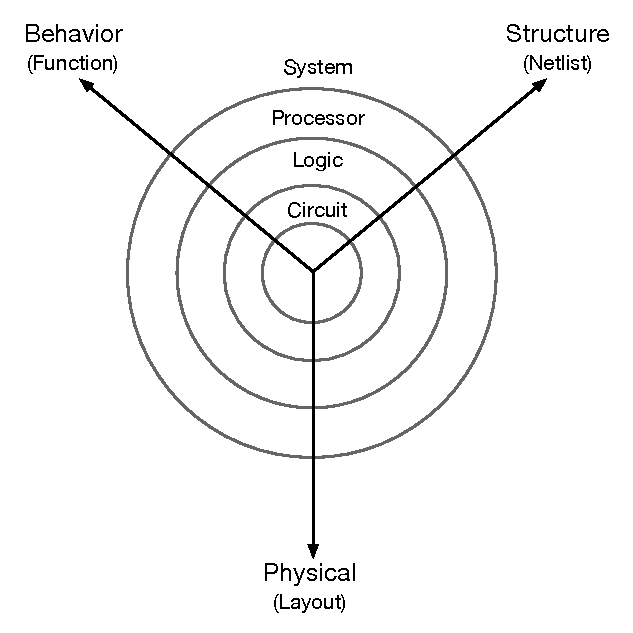
\includegraphics[width=0.5\textwidth]{figures/Introduction/Y-chart.pdf}
    \caption{Y-Chart}
    \label{fig:y-chart}
\end{figure}

Y-Chart divides design representation into three domains:1)Behavioral, it can also called functionality and specification, 2)Structural, also called netlist or a block diagram and 3)Physical, usually called layout or board design. Behavior represents a design as a black-box but it describes the output base on inputs over time. What behavior representation doesn't specify is how the black-box is structured or how to build the black-box. This is the task of structural representation. In this specification, black-box is represented as a set of components and connections. While, it's possible to drive the behavior of black-box from its components and its connections but understanding the behavior can be very difficult since it is obscured by the details of each component and connection.
Eventually, physical design describe different dimension of each component.

The Y-chart also defines multiple level of abstractions for a design by drawing concentric circles on the Y. Typically, four levels are used: system, processor, logic and circuit levels.
The name of each abstraction level is derived from the types of the components generated on that abstraction level.
For instance, on the processor level, we generate standard and custom processors, or special-hardware components such as memory controllers, arbiters, brides and various interface components. At the higher level, system level, we design standard or embedded systems consisting of processors, memories, buses, and other processor components.

Let's look at binary counter as an example. In this example at the algorithmic-level, we only know that at every cycle the input value will be increased by one and the output in the next cycle would be the input plus one.
At the next lower level, we understand that to carry out this function some sort of register is needed to hold the value of the counter.
We can state this idea using a register transfer statement such as $AC \leftarrow AC + 1$.
On the structural side, the register consists of gates and flip-flops, which themselves consist of transistors.

\paragraph{Synthesis:}On each abstraction level, we need a library of components to be used in building \emph{the structure} for a given \emph{behavior}.
This process of converting the given behavior into a structure for a given haviour is called \emph{synthesis}.
On the other hand, if each component in the library is given with its structure and
the physical implementation, we can proceed with physical design.
Thus each component in the library may have up to three different models representing
three different axes in the Y-Chart: behavior or function; structure, which
contains the components from the lower level of abstraction; and the physical.


% \subsection{Hardware Design Methodologies}

% The first two clear advantages of automation of design process is first, it assures a much shorter design cycle, second, it allows for more exploration of different design style since different designs can be generated and evaluated quickly.
% And the ultimate goal of automation process is to out-perform average human designers in generating high quality designs. Another main advantages of synthesis is to capture the designer knowledge so that the process of making follow-on chip(s) is much easier and automated although human quality can be achieved on a single task.

% Currently, there are two schools of toughs to design a hardware. The first school is capture-and-simulation school believes that human designers have very good design knowledge accumulated through experience that \emph{cannot be automated}. In this case, programming FPGAs involves using a combination of vendor-supplied IP blocks, hand tuned hardware modules written using either low-level RTL or high-level synthesis tools, and architecture-specific glue logic to communicate with off-chip components such as DRAM.

% The second school believes to describe the design and high level and synthesis from description. This school believes that a top-down methodology, in which designers describe the intent of the design and automation tool's add detailed structure, would be better suited for the complex designs. This approach focuses on definition of description languages, design models and synthesis algorithms. In this model, designers' intuition can substantially reduce the search through the design space.


% We define design synthesis, broadly speaking, as a translation process from a behavioral description into a structural description.


% \paragraph{Describing Y-Chart here to clarify both thoughts}

% \section{Languages, Design and Technologies}
% Synthesis systems must allow for making design tradeoffs using different design styles for different technologies and design goals.

% Some design methodologies like pipelining can be abstracted into language constructs to provide better understanding and simpler synthesis algorithms.

% Unfortunately, each design can be described or modeled using a single language in several different ways.A

% Similarly, a design implementation is not unique.For each function in the design, there are several design styles suitable for different design goals or constraints.

% HLS still lacks a formalism of the type already developed for layout and logic synthesis. HLS uses formalisms based on several different areas, varying from the programming-language paradigm for the behavioral description to layout models for cost and performance estimation.


% The main problem with a design description is its change with the design over time. At the beginning, the description is vague, with little or no implementation detail. More detail is added as the design evolves, and the level of abstraction is lowered until the design is ready for manufacturing. A language that spans all the levels of abstraction would be desirable from a management point of view but would be too cumbersome to be mastered by designers, who work only on one or two levels of abstractions.

% Furthermore, different members of the design team require different aspects of a design, for reasons of verifiability, testability, reliability, information needed by those experts to one language known to everybody would produce a very rich language in which information for any particular aspect of the design would be difficult to find.


\section{Missing Semantics}

As an example of this problem, we can look in ~\ref{fig:missing_semantics} at a simple case statement available in any hardware or system modeling language.
This type of case statement can be used to model a FSM in which every case such as X1,X2, ..., represents a state in which all its next states are de ned.
This type of case statement can also be used to model a look-up table, in which every case X1, X2, ..., indicates a location in the memory that contains a value in the table.
Therefore,  we can use the same case statement with the same variables  and format to describe two completely different components.
Unfortunately, FSMs and look-up tables require completely different implementations:  a FSM can be implemented with a controller or with logic gates, while a look-up table is usually implemented with some kind of memory.
It is also possible to implement a FSM with a memory or a table using logic gates.
However, this would not bea very ef cient implementation, and it would not be acceptable to any designer.
So a model which uses case statements to model FSMs and tables is good for simulation but not for implementation because neither a designer nor a synthesis tool can determine which type of structure was described by the case statement.
The lesson is that contemporary modeling languages allow modelers to de-scribe the design in many different ways and to use the same description for different designs details. But for automatic refinement, synthesis, and veri cation, we need clean and unambiguous semantic which uniquely represents all the system concepts in a given model.  Such a clean semantic is missing from most of the simulation-oriented  languages.
In order to have well defined semantics, we need to introduce some form of formalism to models and modeling languages.


\begin{figure}[h]
    \centering
    \includegraphics[width=0.7\textwidth]{figures/Introduction/Missing_semantics.pdf}
    \caption{Missing Semantics}
    \label{fig:missing_semantics}
\end{figure}



\section{Hand build application specific accelerators}

\section{Different approaches to HLS}
\subsection{FSM models}
\begin{enumerate}
    \item Legup
    \item Vivado and Intel
\end{enumerate}

\subsection{Elastic circuit}

\begin{enumerate}
    \item CASH
    \item AHL
    \item Elastic circuit
\end{enumerate}

\subsection{DSL types}
\begin{enumerate}
    \item Halide HLS
    \item Spatial
\end{enumerate}

\subsection{Library based}


\section{Chip generators}

This class of hardware design bring configurablity to hand design optimizations. This is critical to use when try to auto generate hardware.
It's also necessary when someone wants to do DSE.
\begin{enumerate}
    \item Genesis
    \item FPTunner
    \item OpenPinto
    \item Modular cores
\end{enumerate}

\subsection{Hardware generator languages}
\begin{enumerate}
    \item Chisel, Firrtl
    \item Rocket core
\end{enumerate}